\documentclass{standalone}
\usepackage{tikz}
\usetikzlibrary{patterns, positioning}
\usepackage[sfdefault]{ClearSans} %% option 'sfdefault' activates Clear Sans as the default text font
\usepackage[T1]{fontenc}

\begin{document}
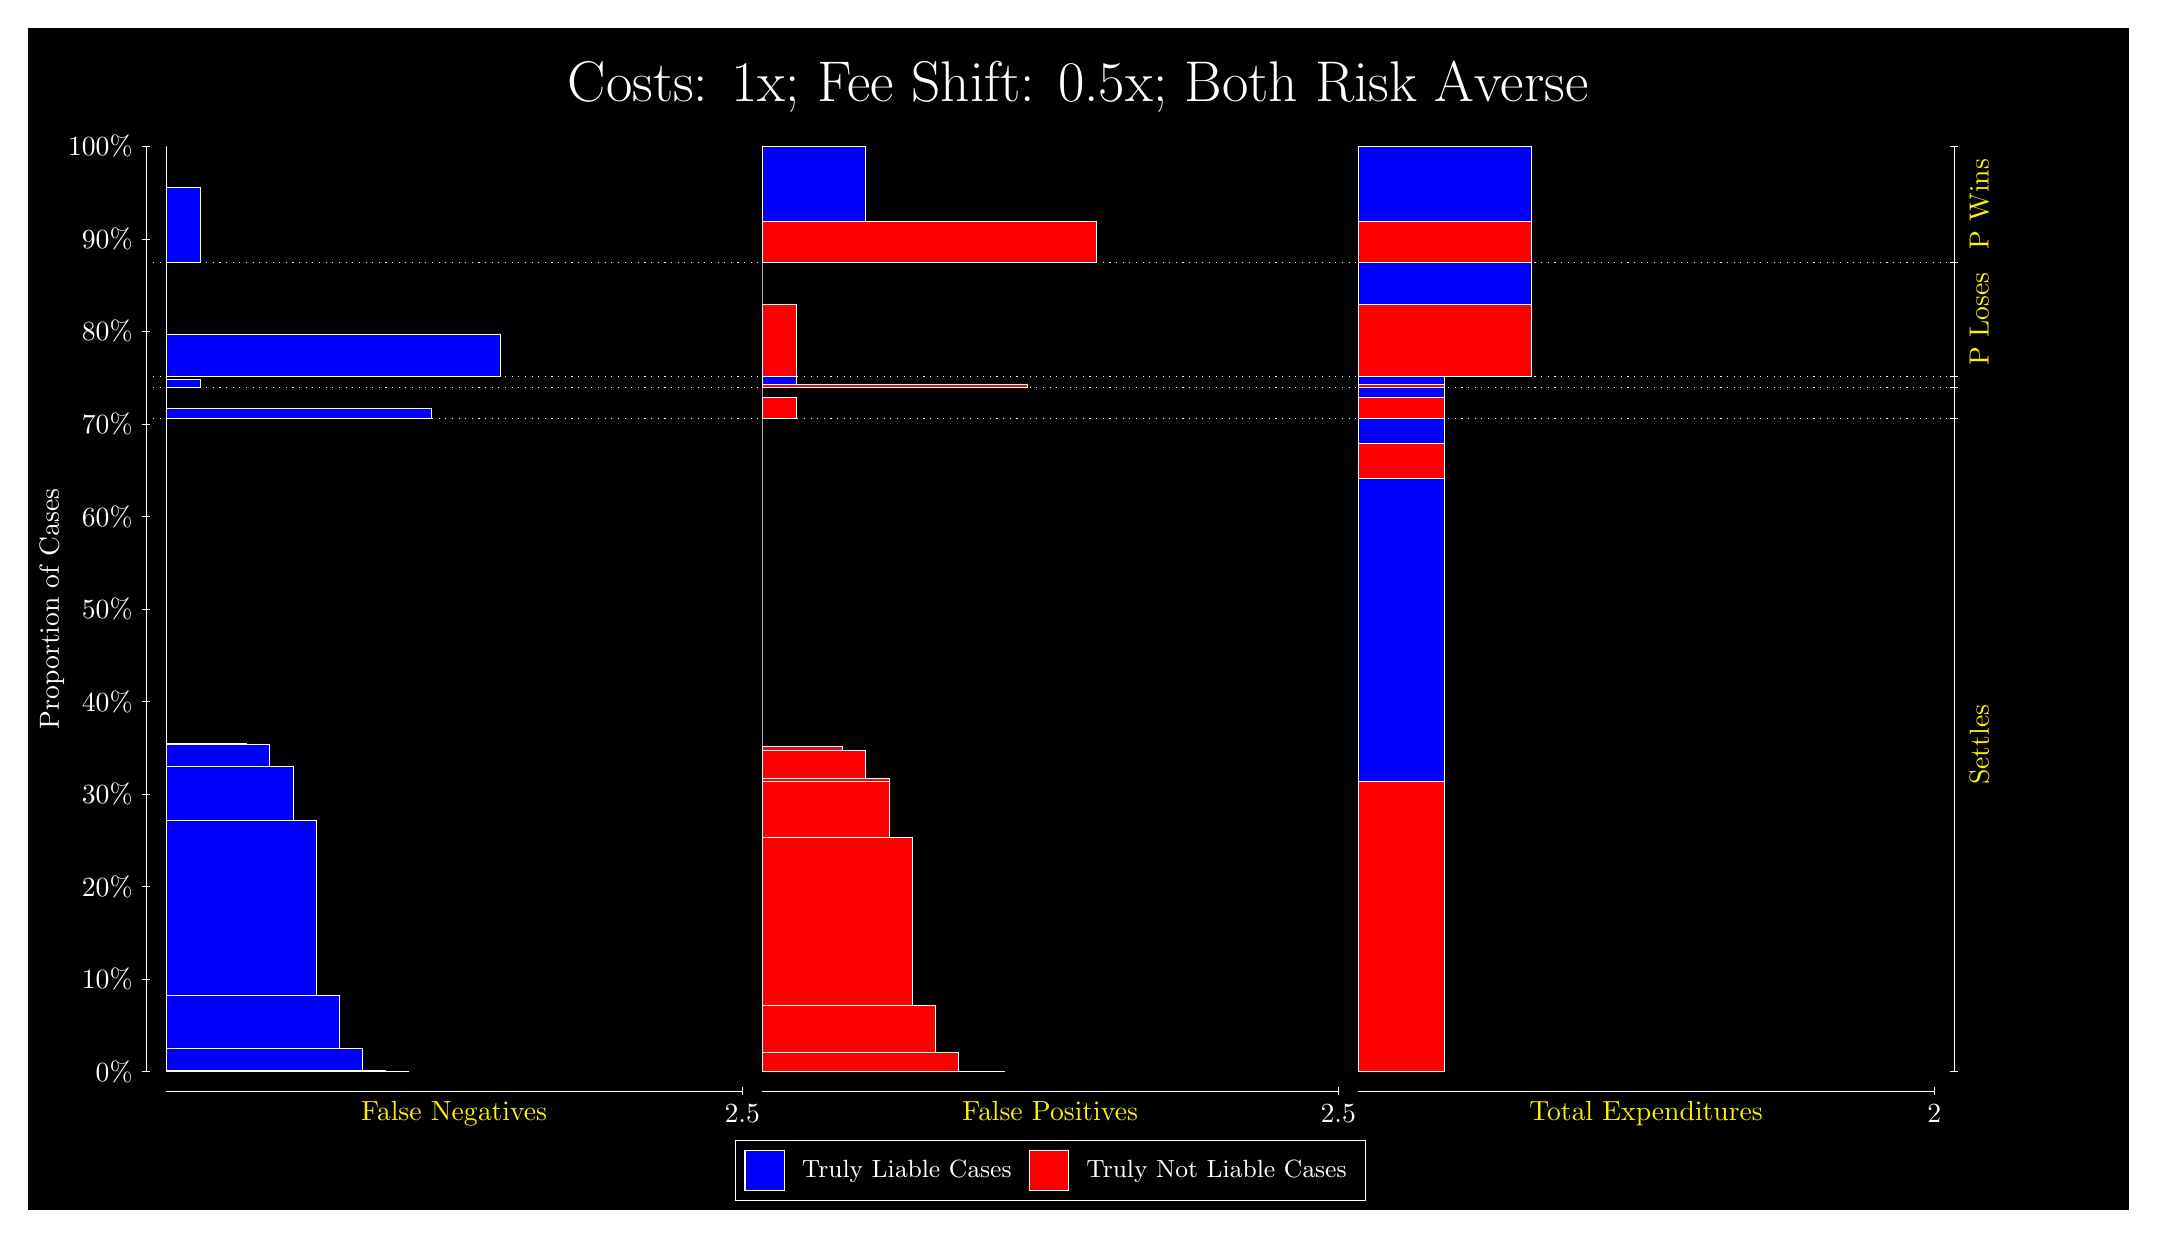
\begin{tikzpicture}
\draw[fill=black] (0,0) rectangle (26.667,15);
\draw[text=white] (0,13.5) rectangle (26.667,15) node[midway] {\huge Costs: 1x; Fee Shift: 0.5x; Both Risk Averse};
\draw[white, very thin] (1.5,1.75) -- (1.5,13.5);
\node[rotate=90, text=white, anchor=center] at (0.3, 7.625) {Proportion of Cases};
\draw[white, very thin] (1.45,1.75) -- (1.55,1.75);
\node[text=white, anchor=east] at (1.45, 1.75) {0\%};
\draw[white, very thin] (1.45,2.925) -- (1.55,2.925);
\node[text=white, anchor=east] at (1.45, 2.925) {10\%};
\draw[white, very thin] (1.45,4.1) -- (1.55,4.1);
\node[text=white, anchor=east] at (1.45, 4.1) {20\%};
\draw[white, very thin] (1.45,5.275) -- (1.55,5.275);
\node[text=white, anchor=east] at (1.45, 5.275) {30\%};
\draw[white, very thin] (1.45,6.45) -- (1.55,6.45);
\node[text=white, anchor=east] at (1.45, 6.45) {40\%};
\draw[white, very thin] (1.45,7.625) -- (1.55,7.625);
\node[text=white, anchor=east] at (1.45, 7.625) {50\%};
\draw[white, very thin] (1.45,8.8) -- (1.55,8.8);
\node[text=white, anchor=east] at (1.45, 8.8) {60\%};
\draw[white, very thin] (1.45,9.975) -- (1.55,9.975);
\node[text=white, anchor=east] at (1.45, 9.975) {70\%};
\draw[white, very thin] (1.45,11.15) -- (1.55,11.15);
\node[text=white, anchor=east] at (1.45, 11.15) {80\%};
\draw[white, very thin] (1.45,12.325) -- (1.55,12.325);
\node[text=white, anchor=east] at (1.45, 12.325) {90\%};
\draw[white, very thin] (1.45,13.5) -- (1.55,13.5);
\node[text=white, anchor=east] at (1.45, 13.5) {100\%};

\draw[white, very thin] (24.457,1.75) -- (24.457,13.5);
\draw[white, very thin] (24.407,1.75) -- (24.507,1.75);
\node[anchor=west] at (24.407, 1.75) {};
\draw[white, very thin] (24.407,10.049) -- (24.507,10.049);
\node[anchor=west] at (24.407, 10.049) {};
\draw[white, very thin] (24.407,10.438) -- (24.507,10.438);
\node[anchor=west] at (24.407, 10.438) {};
\draw[white, very thin] (24.407,10.58) -- (24.507,10.58);
\node[anchor=west] at (24.407, 10.58) {};
\draw[white, very thin] (24.407,12.03) -- (24.507,12.03);
\node[anchor=west] at (24.407, 12.03) {};
\draw[white, very thin] (24.407,13.5) -- (24.507,13.5);
\node[anchor=west] at (24.407, 13.5) {};

\draw[white, very thin, fill=blue] (1.75,1.75) rectangle (4.8239,1.7515);
\draw[white, very thin, fill=blue] (1.75,1.7515) rectangle (4.5312,1.7722);
\draw[white, very thin, fill=blue] (1.75,1.7722) rectangle (4.2384,2.0483);
\draw[white, very thin, fill=blue] (1.75,2.0483) rectangle (3.9457,2.7222);
\draw[white, very thin, fill=blue] (1.75,2.7222) rectangle (3.6529,4.9418);
\draw[white, very thin, fill=blue] (1.75,4.9418) rectangle (3.3602,5.6279);
\draw[white, very thin, fill=blue] (1.75,5.6279) rectangle (3.0674,5.9003);
\draw[white, very thin, fill=blue] (1.75,5.9003) rectangle (2.7746,5.9178);
\draw[white, very thin, fill=blue] (1.75,5.9178) rectangle (2.4819,5.9192);
\draw[white, very thin, fill=red] (1.75,5.9192) rectangle (1.75,10.049);
\draw[white, very thin, fill=blue] (1.75,10.049) rectangle (5.1167,10.172);
\draw[white, very thin, fill=red] (1.75,10.172) rectangle (1.75,10.438);
\draw[white, very thin, fill=blue] (1.75,10.438) rectangle (2.1891,10.541);
\draw[white, very thin, fill=red] (1.75,10.541) rectangle (1.75,10.58);
\draw[white, very thin, fill=blue] (1.75,10.58) rectangle (5.9949,11.114);
\draw[white, very thin, fill=red] (1.75,11.114) rectangle (1.75,12.03);
\draw[white, very thin, fill=blue] (1.75,12.03) rectangle (2.1891,12.976);
\draw[white, very thin, fill=red] (1.75,12.976) rectangle (1.75,13.5);
\draw[white, very thin, fill=red] (9.3189,1.75) rectangle (12.393,1.7511);
\draw[white, very thin, fill=red] (9.3189,1.7511) rectangle (12.1,1.7579);
\draw[white, very thin, fill=red] (9.3189,1.7579) rectangle (11.807,1.993);
\draw[white, very thin, fill=red] (9.3189,1.993) rectangle (11.515,2.5902);
\draw[white, very thin, fill=red] (9.3189,2.5902) rectangle (11.222,4.7188);
\draw[white, very thin, fill=red] (9.3189,4.7188) rectangle (10.929,5.4312);
\draw[white, very thin, fill=red] (9.3189,5.4312) rectangle (10.929,5.4757);
\draw[white, very thin, fill=red] (9.3189,5.4757) rectangle (10.636,5.8356);
\draw[white, very thin, fill=red] (9.3189,5.8356) rectangle (10.344,5.879);
\draw[white, very thin, fill=red] (9.3189,5.879) rectangle (10.051,5.8802);
\draw[white, very thin, fill=blue] (9.3189,5.8802) rectangle (9.4652,5.8816);
\draw[white, very thin, fill=blue] (9.3189,5.8816) rectangle (9.3189,10.049);
\draw[white, very thin, fill=red] (9.3189,10.049) rectangle (9.758,10.316);
\draw[white, very thin, fill=blue] (9.3189,10.316) rectangle (9.3189,10.438);
\draw[white, very thin, fill=red] (9.3189,10.438) rectangle (12.686,10.476);
\draw[white, very thin, fill=blue] (9.3189,10.476) rectangle (9.758,10.58);
\draw[white, very thin, fill=red] (9.3189,10.58) rectangle (9.758,11.495);
\draw[white, very thin, fill=blue] (9.3189,11.495) rectangle (9.3189,12.03);
\draw[white, very thin, fill=red] (9.3189,12.03) rectangle (13.564,12.554);
\draw[white, very thin, fill=blue] (9.3189,12.554) rectangle (10.636,13.5);
\draw[white, very thin, fill=red] (16.888,1.75) rectangle (17.986,5.4312);
\draw[white, very thin, fill=blue] (16.888,5.4312) rectangle (17.986,9.2806);
\draw[white, very thin, fill=red] (16.888,9.2806) rectangle (17.986,9.2818);
\draw[white, very thin, fill=blue] (16.888,9.2818) rectangle (17.986,9.2832);
\draw[white, very thin, fill=red] (16.888,9.2832) rectangle (17.986,9.7311);
\draw[white, very thin, fill=blue] (16.888,9.7311) rectangle (17.986,10.049);
\draw[white, very thin, fill=red] (16.888,10.049) rectangle (17.986,10.316);
\draw[white, very thin, fill=blue] (16.888,10.316) rectangle (17.986,10.438);
\draw[white, very thin, fill=red] (16.888,10.438) rectangle (17.986,10.476);
\draw[white, very thin, fill=blue] (16.888,10.476) rectangle (17.986,10.58);
\draw[white, very thin, fill=red] (16.888,10.58) rectangle (19.083,11.495);
\draw[white, very thin, fill=blue] (16.888,11.495) rectangle (19.083,12.03);
\draw[white, very thin, fill=red] (16.888,12.03) rectangle (19.083,12.554);
\draw[white, very thin, fill=blue] (16.888,12.554) rectangle (19.083,13.5);
\draw[white, dotted] (1.5,10.049) -- (24.457,10.049);
\draw[white, dotted] (1.5,10.438) -- (24.457,10.438);
\draw[white, dotted] (1.5,10.58) -- (24.457,10.58);
\draw[white, dotted] (1.5,12.03) -- (24.457,12.03);
\draw[white, very thin] (1.75,1.5) -- (9.0689,1.5);
\node[text=yellow, anchor=north] at (5.4094, 1.5) {False Negatives};
\draw[white, very thin] (9.0689,1.45) -- (9.0689,1.55);
\node[text=white, anchor=north] at (9.0689, 1.45) {2.5};

\draw[white, very thin] (9.3189,1.5) -- (16.638,1.5);
\node[text=yellow, anchor=north] at (12.978, 1.5) {False Positives};
\draw[white, very thin] (16.638,1.45) -- (16.638,1.55);
\node[text=white, anchor=north] at (16.638, 1.45) {2.5};

\draw[white, very thin] (16.888,1.5) -- (24.207,1.5);
\node[text=yellow, anchor=north] at (20.547, 1.5) {Total Expenditures};
\draw[white, very thin] (24.207,1.45) -- (24.207,1.55);
\node[text=white, anchor=north] at (24.207, 1.45) {2};

\node[text=yellow, centered, rotate=90] at (24.777, 5.8997) {Settles};


\node[text=yellow, centered, rotate=90] at (24.777, 11.305) {P Loses};
\node[text=yellow, centered, rotate=90] at (24.777, 12.765) {P Wins};

\draw (12.978300999999998,1.5) node[draw=none] (baseCoordinate) {};
\begin{scope}[align=center]
        \matrix[scale=0.5, draw=white, below=0.5cm of baseCoordinate, nodes={draw}, column sep=0.1cm]{
            \node[rectangle, draw, minimum width=0.5cm, minimum height=0.5cm, fill=blue] {}; &
            \node[draw=none, font=\small, text=white] (B) {Truly Liable Cases}; &
            \node[rectangle, draw, minimum width=0.5cm, minimum height=0.5cm, fill=red] {}; &
            \node[draw=none, font=\small, text=white] (B) {Truly Not Liable Cases}; \\
            };
\end{scope}

\end{tikzpicture}
\end{document}